\documentclass[a4paper,12pt]{article}
\usepackage[fleqn]{amsmath}
\usepackage{amssymb}
\usepackage{graphicx}
\graphicspath{ {./images/} }
\begin{document}

\title{Data Distribution}	
\author{Edward Jex}
\maketitle
Data can be distributed due to its appearance to help us interpret the spread of data. \\
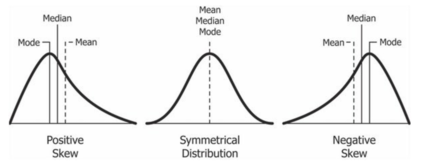
\includegraphics[scale=1.5]{SkewedData} \\
Data can also be bimodal, meaning it has two peaks \\
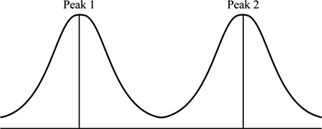
\includegraphics[scale=0.7]{Bimodal} \\

\section*{Measures of Central Tendency}
There are four measures of central tendency that we should be aware of:
\begin{itemize}
	\item Mode - The mode is the value that occurs most frequently. The distribution is uni-modal if there is only one mode. If two non-adjacent values occur mode frequently than the rest, the distribution is said to be bi-modal, even if the frequencies aren't the same. 
	\item Medial - It is the middle value. It is a good measure as it isn't skewed as much by outliers but most representative for symmetrical data. 
	\item Mean - Found by adding all the values together and dividing by the number of values. We use the symbol $\bar{x}$ to denote the mean. It is the best measure for skewed data but also representative for symmetrical data. It is affected by outliers. 
	\item Midrange - This is the average of the highest and lowest values. It is easy to calculate but only useful when the data is symmetrical and contains no outliers. 
\end{itemize}

\section*{Measures of Spread}
There are three measures of spread we need to know about which help us talk about how varied the data is.
\begin{itemize}
	\item Range - This is the highest subtract the lowest. Again this is not useful if we have any outliers.
	\item Interquartile Range - As seen before. We can also find the semi-interquartile range which is half the interquartile range.
	\item Standard Deviation - This we will learn about separately but is the most widely used measure of spread.   
\end{itemize}

\section*{Standard Deviation}
Why is it useful?
\begin{itemize}
	\item Approximately 68\% of values lie within 1 standard deviation of the mean. 
	\item 95\% lie within 2
\end{itemize}
If you have a particular values which is more than two standard deviations from the mean it should be investigated as a possible outlier. \\
\begin{align*}
\text{Sum of Squares } & = S_{xx} \\ 
& = \sum x^2 - n\bar{x}^2 \\
& = \sum x^2 - \frac{(\sum x)^2}{n} \\
\end{align*}
The variance is found by $var = s^2 = \frac{s_{xx}}{n-1}$ \\
The standard deviation is found by the square root of the variance. \\
$s = \sqrt{\frac{s_{xx}}{n-1}} = \sqrt{var}$

\subsubsection*{Example 1}
Find the standard deviation of 0, 1, 0, 3, 0, 2
\begin{align*}
\bar{x} & = \frac{1 + 2 + 3}{6} = 1 \\
s_{xx} & = (0^2 + 1^2 + 0^2 + 3^2 + 0^2 + 2^2) - 6 \times 1^2
& = 14-6 = 8 \\
s & = \sqrt{\frac{s_{xx}}{n-1}} \\
& = \sqrt{\frac{8}{5}} = 1.26 \\
\end{align*}

\subsection*{Frequency tables}
If you have a frequency table, we can still work out the standard deviation. The only thing that changes is our formula for sum of squares: \\
$s_{xx} = \sum x^2f - n\bar{x}^2$ \\

\end{document}